\documentclass{article}

\usepackage{graphicx}
\usepackage{fancyhdr}
\usepackage[sorting=none]{biblatex}
\usepackage[margin=1in]{geometry}
\usepackage{listings}
\usepackage[hidelinks]{hyperref}
\usepackage{xcolor}
\usepackage{xepersian}
\usepackage{ltablex}
\usepackage{booktabs, makecell, longtable}



\addbibresource{bibliography.bib}
\settextfont[Scale=1.2]{IRNazli.ttf}
\setlatintextfont[Scale=1]{times.ttf}
\renewcommand{\baselinestretch}{1.5}
\pagestyle{fancy}
\fancyhf{}
\renewcommand{\headrulewidth}{1pt}
\renewcommand{\footrulewidth}{1pt}
\setcounter{tocdepth}{1}
\begin{document}

\def\by{نگارش}
\def\superv{مدرس}
\def\faculty{دانشکده مهندسی کامپیوتر}
\def\course{رایانش عصبی}
\def\docTitle{پروژه پنجم }
\def\supervisor{دکتر رضا صفابخش}
\def\fname{سیدمهدی }
\def\lname{میرفندرسکی}
\def\stuNum{401131065}
\def\docDate{دی 1401}

\rhead{\docTitle}
\lhead{درس \course}
\rfoot{\fname \lname}
\lfoot{\stuNum}
\cfoot{\\ \thepage}



\begin{titlepage}
\begin{center}
%
\includegraphics[width=0.4\textwidth]{fa-logo.png}\\
\centerline{{
\includegraphics[height=3.8cm]{fa-logo}}}        
\LARGE
%\textbf{دانشگاه صنعتی اصفهان}\\
%\textbf{دانشکده مهندسی کامپیوتر}\\
\bf{\fontsize{16pt}{16pt}\selectfont دانشگاه صنعتی امیرکبیر}\par
\fontsize{14pt}{15pt}\selectfont(پلی‌تکنیک تهران)\par
\fontsize{16pt}{17pt}\selectfont \faculty \par
        
\par
        

\vfill
{\huge\settextfont{B_Titr.ttf}{\docTitle  درس  \course}}
\vfill
 
\settextfont[Scale=1.2]{BNazanin.ttf}
{\huge\by}\\
\fontsize{18pt}{19pt}\selectfont\bfseries{\fname \lname} \\
\settextfont[Scale=1.2]{BNazanin.ttf}
{\huge\superv}\\
{\fontsize{18pt}{19pt}\selectfont\bfseries\par\supervisor}\\
\fontsize{16pt}{17pt}\selectfont\docDate\\
 
 
        
\LARGE
%\textbf{نام و نام خانوادگی: مجید فرهادی}\\
%\textbf{شماره دانشجویی: 9700000}\\
%\textbf{نیم‌سال تحصیلی: پاییز 1400}\\
%\textbf{مدرّس: دکتر محمّدرضا حیدرپور}\\
%\textbf{دستیاران آموزشی: مجید فرهادی - دانیال مهرآیین - محمّد نعیمی}\\
\end{center}
\end{titlepage}


\tableofcontents

\newpage



\section{سوال اول}
اساسا با این کار به نوعی می‌توانیم داده‌های سری زمانی را به یک مسئله یادگیری نظارت‌شده یا بدون نظارت تبدیل کنیم. در واقع در نظر گرفتن لگ‌ها در تجزیه و تحلیل سری‌های زمانی بسیار مفید هستند زیرا در بین داده‌های سری زمانی خودهمبستگی وجود دارد که همبستگی مقادیر درون یک سری زمانی با مقادیر قبلی خود است. البته بسته به مسئله هرچه از داده فعلی دور شویم، امکان دارد این همبستگی کم یا زیاد شود. با این کار در این مسئله، مشخص می‌کنیم که شبکه نسبت به چقدر داده‌های قبلی حساس باشد. به عنوان مثال احتمالا در مسئله بورس بیشتر از شش ماه گذشته وابستگی نخواهند داشت.

در ادامه برای حل این بخش تعداد گام‌های ورودی برابر با 32 و همچنین با \lr{offset} یک، پنجره‌ها ایجاد شدند. عدد 32 بدین دلیل بود که تاریخچه نزدیک به یک ماه درنظر گرفته شود.

% -------------------------------------------------------------------

\section{سوال دوم}
برای آموزش شبکه تلاش‌های بسیاری صورت گرفت اما نتایج قابل قبولی دریافت نشد. درنهایت معماری انتخاب شده بدین صورت است که یک لایه \lr{SimpleRNN}، یک لایه \lr{Dense} و در نهایت یک تک نورون برای مسئله دسته‌بندی در نظر گرفته شد. درضمن تابع فعالیت خروجی شبکه‌ها سیگموید و توابع فعلیت لایه‌های دیگر \lr{relu} درنظر گرفته شد. همچنین سایز دسته برابر 16 و ای‌پاک برابر با 10 درنظر گرفته شد. مشابه تمرینات قبل کالبک زیر نیز گذاشته شد.

\lr{es-callback = EarlyStopping(monitor="val-loss", patience=3, restore-best-weights=True)}

در جدول زیر ترکیبات مختلف تعداد واحدها مشاهده می‌شود.

\begin{table}[!h]
    \centering
    \begin{tabular}{|c|c|c|c|c|c|}
    \hline
    شماره & \lr{SimpleRNN} & \lr{Dense} & آموزشی صحت & اعتبارسنجی صحت & تست صحت \\ \hline
    1 & 1 & 16 & $58.57$ & $58.17$ & $58.03$ \\ \hline
    2 & 2 & 16 & $58.57$ & $58.17$ & $58.03$ \\ \hline
    3 & 3 & 16 & $58.57$ & $58.17$ & $58.03$ \\ \hline
    4 & 4 & 16 & $56.52$ & $62.5$ & $57.79$ \\ \hline
    5 & 5 & 16 & $59.05$ & $59.13$ & $57.79$ \\ \hline
    6 & 6 & 16 & $58.57$ & $58.17$ & $58.03$ \\ \hline
    7 & 7 & 16 & $59.12$ & $58.65$ & $57.55$ \\ \hline
    8 & 1 & 32 & $58.57$ & $58.17$ & $58.03$ \\ \hline
    9 & 2 & 32 & $58.78$ & $58.65$ & $57.55$ \\ \hline
    10 & 3 & 32 & $58.85$ & $58.65$ & $58.03$ \\ \hline
    11 & 4 & 32 & $58.57$ & $58.17$ & $58.03$ \\ \hline
    12 & 5 & 32 & $59.05$ & $61.54$ & $61.15$ \\ \hline
    13 & 6 & 32 & $58.57$ & $58.17$ & $58.03$ \\ \hline
    14 & 7 & 32 & $58.57$ & $58.17$ & $58.03$ \\ \hline
    15 & 1 & 64 & $58.57$ & $58.17$ & $58.03$ \\ \hline
    16 & 2 & 64 & $58.5$ & $62.02$ & $59.71$ \\ \hline
    17 & 3 & 64 & $58.64$ & $58.65$ & $57.79$ \\ \hline
    18 & 4 & 64 & $58.85$ & $58.65$ & $57.55$ \\ \hline
    19 & 5 & 64 & $58.57$ & $58.17$ & $58.03$ \\ \hline
    20 & 6 & 64 & $58.98$ & $57.69$ & $58.99$ \\ \hline
    21 & 7 & 64 & $60.29$ & $60.1$ & $59.23$ \\ \hline
    22 & 1 & 128 & $58.57$ & $58.17$ & $58.03$ \\ \hline
    23 & 2 & 128 & $58.57$ & $58.17$ & $58.03$ \\ \hline
    24 & 3 & 128 & $58.57$ & $58.17$ & $58.03$ \\ \hline
    25 & 4 & 128 & $58.23$ & $60.1$ & $60.43$ \\ \hline
    26 & 5 & 128 & $57.89$ & $60.58$ & $60.19$ \\ \hline
    27 & 6 & 128 & $58.5$ & $61.54$ & $61.15$ \\ \hline
    28 & 7 & 128 & $57.61$ & $62.5$ & $58.03$ \\ \hline



\end{tabular}
\end{table}


\cleardoublepage

با در نظر گرفتن صحت محموعه آموزشی و اعتبارسنجی معماری زیر انتخاب شد:

\begin{table}[!h]
    \centering
    \begin{tabular}{|c|c|c|c|c|c|}
    \hline
    شماره & \lr{SimpleRNN} & \lr{Dense} & آموزشی صحت & اعتبارسنجی صحت & تست صحت \\ \hline
    16 & 2 & 64 & $58.5$ & $62.02$ & $59.71$ \\ \hline

\end{tabular}
\end{table}


همچنین نمودار صحت و خطای مجموعه آموزشی و اعتبارسنجی برای بهترین معماری در ادامه مشاهده می‌شود.

\begin{figure}[!h]
    \centering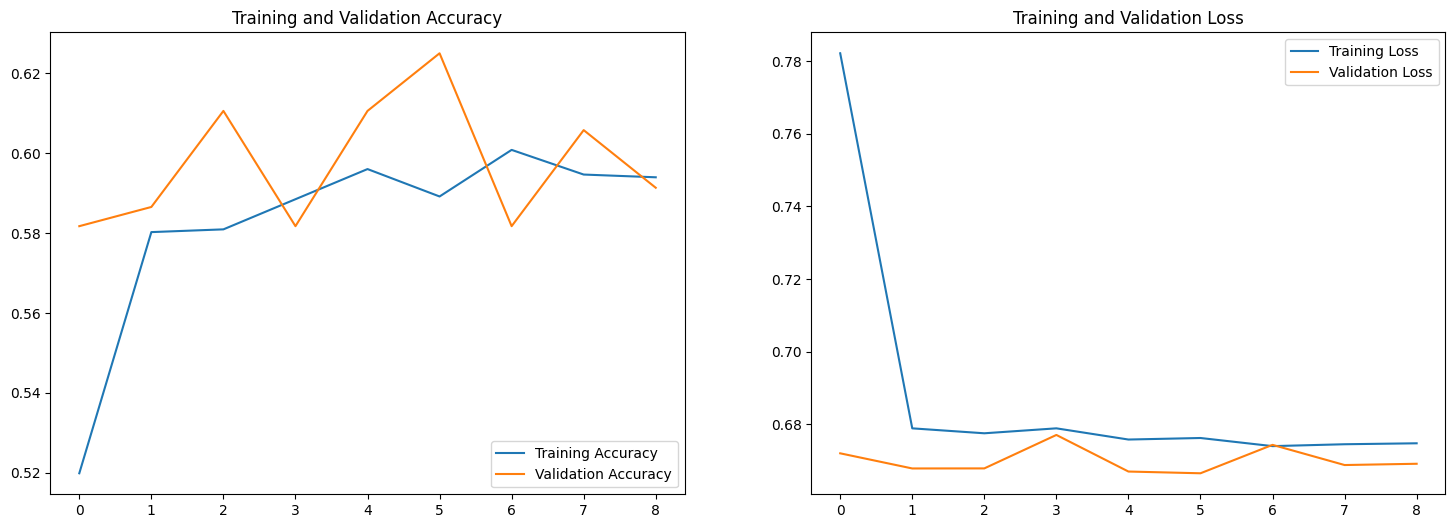
\includegraphics[scale=.40]{./p2-1}
    \caption{نمودار صحت و خطای بهترین معماری}\label{fig.21}
\end{figure}

\cleardoublepage

% -------------------------------------------------------------------

\section{سوال سوم}
برای این بخش یک مدل شبکه کانولوشنی آموزش دیده شد. توجه شود که برای این قسمت سعی و خطا در نظر گرفته نشده است (سعی و خطا شبکه کانولوشنی در پروژه چهارم). معماری شبکه طراحی شده و نتایج آن در ادامه مشاهده می‌شود.

\begin{figure}[!h]
    \centering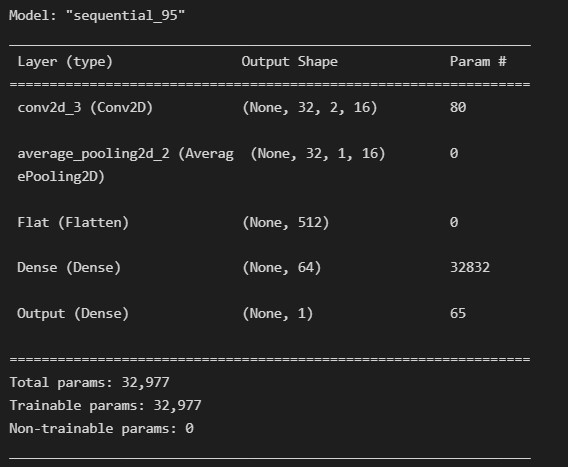
\includegraphics[scale=.55]{./p3-1}
    \caption{معماری شبکه کانولوشنی}\label{fig.31}
\end{figure}

\begin{figure}[!h]
    \centering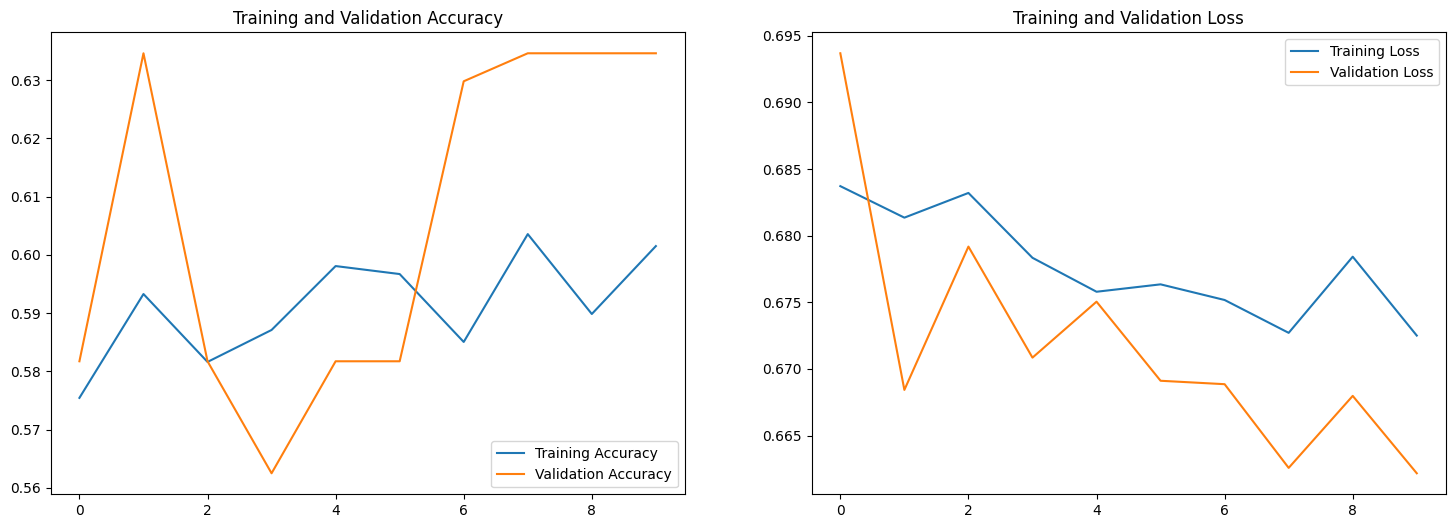
\includegraphics[scale=.40]{./p3-2}
    \caption{نمودارهای شبکه کانولوشنی}\label{fig.32}
\end{figure}

\cleardoublepage

همانطور که مشاهده می‌شود این شبکه کانولوشنی تقریبا در حد بهترین شبکه قسمت قبل عمل کرده است (می‌توان گفت کانولوشنی حتی مقداری بهتر عمل کرده است.) . همچنین احتمالا با سعی و خطا بتوان نتایج بهتری را نیز کسب کرد. پس در کل اینگونه برداشت شد که شبکه کانولوشنی برای این مسئله بهتر عمل می‌کند.

% -------------------------------------------------------------------

\section{سوال چهارم}
در این گزارش ابتدا انواع ناهنجاری‌ها بیان شده است: (داده‌های پرت افزایشی، تغییرات زمانی و تغییر سطح یک پدیده). در ادامه مجموعه داده قیمت بیتکوین برای ادامه کار درنظر گرفته شده است. سپس مجموعه آموزشی و تست را ایجاد و آن‌ها را با یک روش یکسان نرمالایز کرده است. در نهایت برای آخرین قسمت پیش‌پردازش مقدار لگ 30 برای آموزش انتخاب شده است. سپس شبکه خود کدگذاری با معماری زیر شامل لایه کانولوشنی و \lr{LSTM} طراحی کرده است. سپس به آموزش شبکه پرداخته شد (بوضوح ورودی و خروجی شبکه داده‌های آموزشی هستند). سپس مشابه تمارین گذاشته با نمودارهای خطای آموزش و اعتبارسنجی، بایاس و واریانس مدل را بررسی می‌کند. حال که مدل از نظر بایاس و واریانس مطلوب است، نوبت به محاسبه خطای بازسازی کل شبکه خود کدگذار می‌رسد. در این مرحله خطای بازسازی داده‌های آموزشی و تست محاسبه می‌شوند. در داده‌های تست اگر مقداری از حداکثر مقدار خطای آموزشی (\lr{mae}) بیشتر باشد، در لیست ناهنجاری‌ها ذخیره می‌شود (اساس این روش بر این اساس است که اگر داده‌ای از تست بازسازی مناسبی نداشت به عنوان ناهنجاری شناخته شود.).

\begin{figure}[!h]
    \centering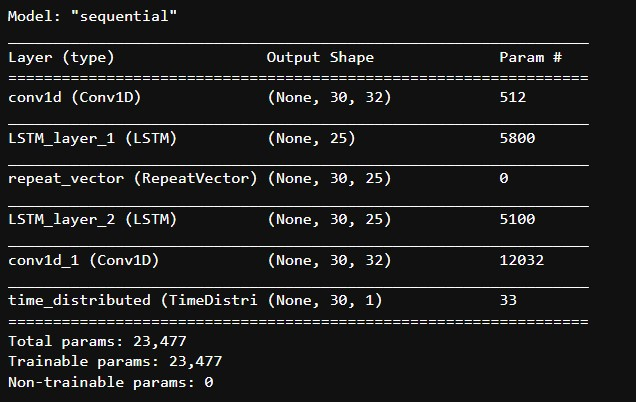
\includegraphics[scale=.55]{./p4-1}
    \caption{معماری سوال چهارم}\label{fig.41}
\end{figure}
% -------------------------------------------------------------------

\section{سوال پنجم}
این مقاله از شبکه‌های خود کدگذار برای یادگیری خود نظارتی در مسائل بینایی ماشین استفاده کرده است. بدین صورت که ابتدا یک شبکه‌ خود کدگذار نامتقارن با قسمت کدگذار با پارمترهای بیشتر در نظر گرفته است. سپس به صورت تصادفی بعضی پیکسل‌های ورودی را ماسک (صفر) کرده است. البته کار متمایزی که این مقاله انجام داده است این است که حدود 75 درصد ورودی را ماسک کرده است و 25 درصد باقی مانده را جهت آموزش به شبکه خودکدگذار وارد کرده است. که همین امر باعث افزایش سرعت شده است. و درنهایت وقتی آموزش شبکه به اتمام رسید. ماسک‌های تصاویر تنها به قسمت کدگشای شبکه داده می‌شود تا تصویر بازسازی شود. این ایده کمک بسیار زیادی به تکمیل تصاویر ناقص می‌کند. نکته قابل توجه این خواهد بو.د که داده‌های ماسک شده امکان ورود به کدگذار را نخواهند داشت و تنها باید به قسمت کدگشا وارد شود.

% -------------------------------------------------------------------

\end{document}